\lesson{17 Sep 2024}{Scheduler activation}

\begin{definition}
The paper proposes a kernel interface and \textcolor{gray}{user space} thread package that jointly provide kernel thread functionalities.
\end{definition}

The paper is motivated as follows:

\begin{itemize}
    \item User-level threads built on process abstraction are susceptible to performance degradation \textcolor{gray}{and even incorrect behavior}
    \item User-level threads built on thread abstraction suffered from system integration issues, e.g., to exploit multi-processor
    \item Both the user-level thread library and OS kernel need scheduling information from one another for ``better" decision
\end{itemize}

Kernel threads are inappropriate for support user-level threads. \textit{Scheduler activation} is invented to accommodate the aforementioned problems.

\subsection{Upcall}

\begin{definition}[Scheduler activation]
Scheduler activation (SA) is a kernel mechanism that

\begin{itemize}
    \item serves as an execution context for running user-level threads;
    \item notifies user space thread scheduler of relevant kernel events;
    \item provides space for saving processor context of user-level threads
\end{itemize}
\end{definition}

SA data structure resembles that of a kernel thread, i.e,

\begin{itemize}
    \item a kernel stack for syscall;
    \item a user-level thread for scheduler to map user-level thread to SA;
    \item a control block to record SAs whose threads are blocked or preempted.
\end{itemize}

Each user-level stack holds its own stack\footnote{C++ coroutine is \textbf{stackless}.}.

Kernel events are passed to user space via SA \textit{upcall}. An upcall can be

\begin{figure}[H]
\centering
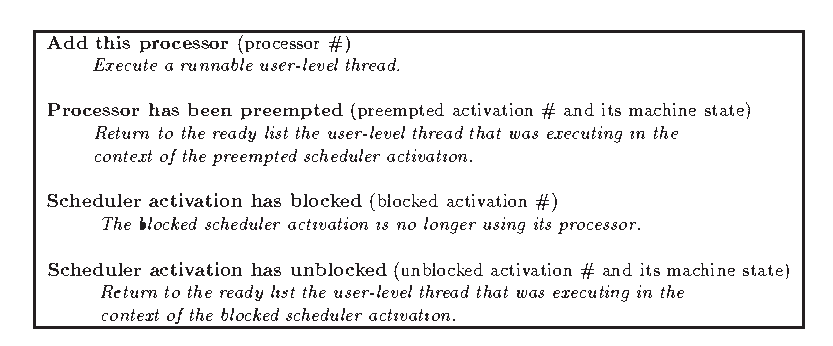
\includegraphics[width=1\linewidth]{figures/upcall.eps}
\end{figure}

As a process starts, OS kernel creates a SA, assigns a processor, and upcalls it to user address space. OS kernel may create more SAs or notify address space of kernel events via the above upcalls.

\begin{note}
A SA is different from a kernel in that a stopped thread \textbf{never} resumes directly. A \textbf{new} SA is always created to notify address space of such a stop.
\end{note}

SAs can be \textbf{reused} by address space to run other threads from the ready list.

\begin{prop}
OS kernel maintains the invariant that there are as many \textbf{running} SAs as processors assigned to the address space.
\end{prop}

\begin{note}
SA is \textbf{unaware} of user space concurrency model. One may build any such model, e.g., worker and future, atop SA \textbf{flexibly}.
\end{note}

\begin{example}
I/O request and completion

\begin{figure}[H]
\centering
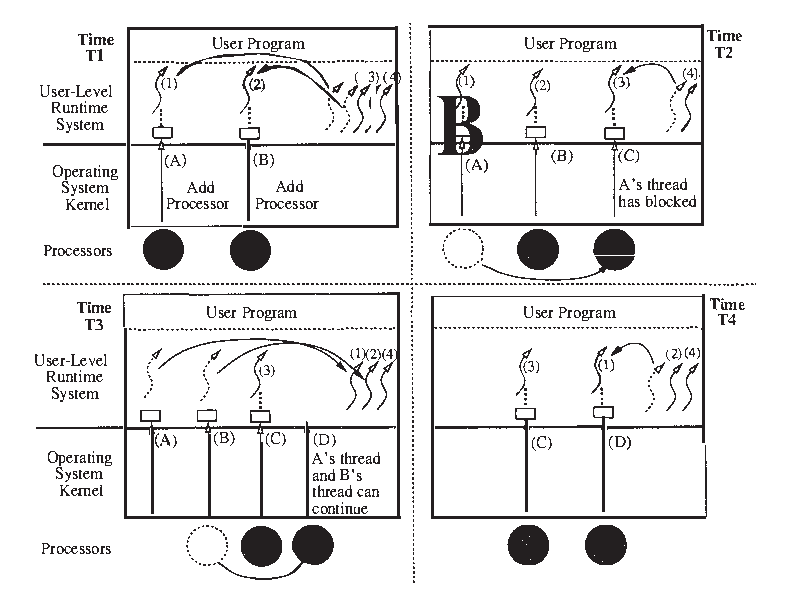
\includegraphics[width=1\linewidth]{figures/sa.eps}
\end{figure}

When thread A blocks at time T2 due to I/O, OS kernel takes the processor that ran thread A, creates a \textbf{new} SA, and notifies address space of the \textcolor{gray}{block} event. \\

When thread A's I/O completes at time T3, OS kernel preempts thread B, creates a \textbf{new} SA, an notifies address space that threads A and B are ready.
\end{example}

In case there are thread priority, use an additional preemption to, e.g., run a previously blocked thread once I/O completes. SA functions properly even though there is a preemption or a page fault in the user-level thread \textbf{manager}.

\subsection{Downcall}

The user-level thread system tells SA a limited subset of events that \textbf{affects SA processor allocation decision}.

\begin{figure}[H]
\centering
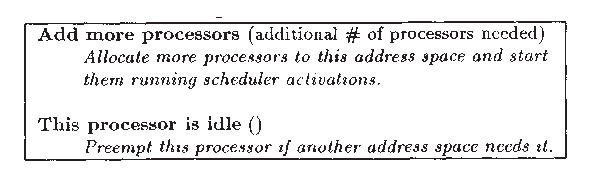
\includegraphics[width=0.7\linewidth]{figures/downcall.eps}
\end{figure}

The above syscalls are made upon state transition when

$$
\begin{matrix}
\text{no. of runnable threads} > \text{no. of processors} \\
\text{no. of runnable threads} < \text{no. of processors}
\end{matrix}
$$

respectively. In the former scenario, OS kernel may search for \textbf{another} address space for idle processor(s). \\

An application may be \textbf{dishonest} about how many processors are busy. This is not unique for SA. OS kernel may favor address space demanding fewer processors or use multi-level feedback to encourage honest feedback.

\begin{example}
Critical section \\

When a thread is preempted, adopt \textit{recovery}\footnote{Another solution is based on \textit{prevention}, which is susceptible to poor performance and deadlock. The paper dispensed with this method.} to

\begin{enumerate}
    \item check if it is in a critical section;
    \item if so, continue running the thread via user-level context switch; otherwise, proceed to step 4 \item the thread runs until it exits the critical section;
    \item relinquish control back to the original upcall \textcolor{gray}{via another user-level context switch}.
\end{enumerate}

Along with implementation techniques, the above mechanism prevents performance degradation.
\end{example}

The proposed SA and user-level thread library is significantly faster than \textcolor{gray}{Ultrix} processes and \textcolor{gray}{Topaz} kernel threads, but slightly \textbf{worse} than na\"ive user-level threads \textcolor{gray}{(FastThreads)} due to state checking in thread library and dynamic SA de/allocation.
